\documentclass{beamer}

% --- TEMA ȘI CULORI ---
\usetheme{Madrid} % Sau 'Berlin', 'Frankfurt', 'Metropolis'
\usecolortheme{beaver} % Schemă de culori (Roșu/Gri)

% --- PACHETE NECESARE ---
\usepackage[utf8]{inputenc}
\usepackage[romanian]{babel}
\usepackage{graphicx}
\usepackage{tikz}
\usetikzlibrary{shadows, positioning, arrows.meta, calc, shapes, fit, backgrounds}

% --- INFORMAȚII TITLU ---
\title[Kerberos]{Kerberos: Un serviciu de autentificare pentru sisteme Open Network}
\subtitle{Proiect Final - Sisteme Distribuite}
\author[Echipa Kerberos]{Prioteasa Liviu Florentin \and Rizescu Iulian Ştefan \and Ţacu Ştefan Darius}
\institute[FMI]{Facultatea de Matematică și Informatică, Universitatea din București}
\date{Ianuarie 2026}

\begin{document}

% Slide 1: Titlu și Echipă
\begin{frame}
  \titlepage
\end{frame}

\begin{frame}{Context și Problemă}
  % Partea de Context
  \begin{itemize}
    \item \textbf{Context:} Tranziția de la sisteme monolitice (acces \textit{Serial/Local}) la sisteme distribuite (acces prin \textit{Rețea}).
  \end{itemize}

  \vspace{0.5cm}

  % Partea de Problemă (Listă încapsulată)
  \begin{block}{Problema: Mediul "Open Network" este nesigur}
    \begin{itemize}
      \item \textbf{Sniffing:} Atacatorii pot intercepta pachetele de date care circulă pe cablu/Wi-Fi.
      \item \textbf{Spoofing:} Adresele IP nu sunt o dovadă suficientă a identității (pot fi falsificate).
    \end{itemize}
  \end{block}

  \vspace{0.5cm}

  % Întrebarea Cheie (Evidențiată distinct)
  \begin{alertblock}{Întrebare Cheie}
    Cum demonstrăm identitatea unui utilizator fără a trimite parola în clar prin rețea?
  \end{alertblock}
\end{frame}

\begin{frame}{Soluția - Trusted Third Party (TTP)}

  % Conceptul de bază
  \begin{block}{Concept}
    Introducerea unei autorități centrale de încredere, denumită \textbf{KDC (Key Distribution Center)}.
  \end{block}

  \vspace{0.5cm}

  % Rolurile sistemului
  \textbf{Roluri și Arhitectură:}
  \begin{itemize}
    \item \textbf{Elimină redundanța riscantă:} Nu mai este necesar ca fiecare server din rețea să stocheze parolele utilizatorilor.
    \item \textbf{Fortificare:} Centralizează administrarea securității într-un singur punct critic, care poate fi protejat intens.
  \end{itemize}

  \vspace{0.5cm}

  % Elementul Cheie (SSO) - Evidențiat
  \begin{alertblock}{Element Cheie}
    Utilizatorul se autentifică o singură dată (\textbf{Single Sign-On}) și primește "bilete" (\textit{Tichete}) pe care le folosește ulterior, fără a mai introduce parola.
  \end{alertblock}

\end{frame}

\begin{frame}{Faza 1: Autentificarea Inițială (AS Exchange)}

  \begin{columns}[c] % Aliniere verticală pe centru

    % --- COLOANA STÂNGA (Text) ---
    \begin{column}{0.5\textwidth}
      \begin{itemize}
        \item \textbf{Scop:} Obținerea "Permisului Universal" (\textbf{TGT} - Ticket Granting Ticket).
        \item \textbf{Mecanism:}
              \begin{itemize}
                \item Utilizator $\rightarrow$ AS: Trimite cererea (ID).
                \item AS $\rightarrow$ Utilizator: Răspunde cu TGT-ul criptat (folosind cheia TGS).
              \end{itemize}
      \end{itemize}

      \vspace{0.3cm}

      % Evidențiem securitatea ca la slide-ul 5
      \begin{alertblock}{Detaliu de Securitate}
        Parola utilizatorului este folosită \textbf{doar local} pentru a decripta răspunsul. Ea nu este trimisă niciodată prin rețea.
      \end{alertblock}
    \end{column}

    % --- COLOANA DREAPTA (Diagrama) ---
    \begin{column}{0.5\textwidth}
      \begin{figure}
        \centering
        % Scalăm diagrama la lățimea coloanei curente
        \resizebox{\linewidth}{!}{%
          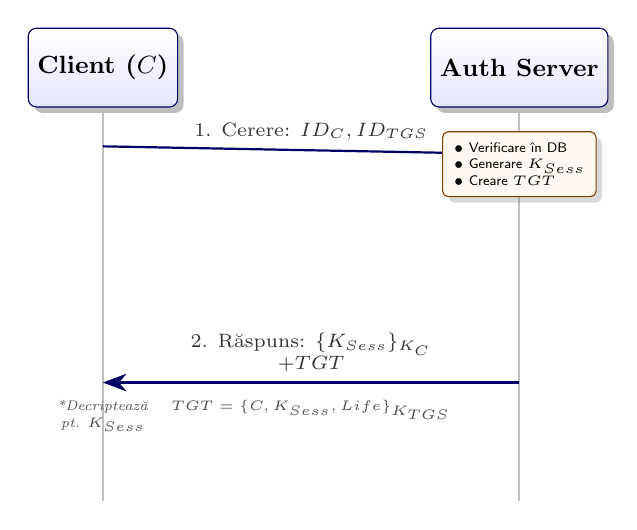
\begin{tikzpicture}[
        node distance=3.2cm, % Distanță compactă, identică cu TGS
        % --- DEFINIȚII DE STIL (Copy-Paste din TGS pentru consistență) ---
        % 1. Actorii (Client/Server): Gradient Albastru + Umbră
        entity/.style={
                draw=blue!40!black,
                top color=white,
                bottom color=blue!10,
                rounded corners=3pt,
                align=center,
                minimum height=1cm,
                minimum width=1.8cm,
                drop shadow,
                font=\bfseries\small
            },
        % 2. Mesajele de pe săgeți
        msg/.style={
                midway,
                above,
                font=\scriptsize,
                color=black!80
            },
        % 3. Notele Interne (Chenar): Galben pal + Border Portocaliu
        process/.style={
                draw=orange!50!black,
                fill=orange!5,
                rounded corners=2pt,
                align=left,
                font=\tiny\sffamily,
                inner sep=4pt,
                drop shadow={opacity=0.3}
            },
        % 4. Formulele Matematice de sub săgeți
        mathnote/.style={
                below=0.1cm,
                font=\tiny,
                color=black!70
            }
    ]

    % 1. Actorii
    \node[entity] (client) {Client ($C$)};
    \node[entity, right=of client] (as) {Auth Server};

    % 2. Liniile vieții
    \draw[thick, gray!50] (client) -- ++(0,-5.5) coordinate (c_end);
    \draw[thick, gray!50] (as) -- ++(0,-5.5) coordinate (as_end);

    % 3. Mesajul 1 (Cerere)
    \draw[-{Stealth[length=3mm]}, thick, color=blue!40!black]
    ($(client)+(0,-1)$) --
    node[msg] {1. Cerere: $ID_C, ID_{TGS}$}
    ($(as)+(0,-1.1)$);

    % --- CHENARUL CERUT (Procesare Internă AS) ---
    % Folosim stilul 'process'
    \node[process, below=0.3cm of as, anchor=north] {
        $\bullet$ Verificare în DB\\
        $\bullet$ Generare $K_{Sess}$\\
        $\bullet$ Creare $TGT$
    };

    % 4. Mesajul 2 (Răspuns)
    \draw[-{Stealth[length=3mm]}, thick, color=blue!40!black]
    ($(as)+(0,-4)$) --
    node[msg, align=center] {2. Răspuns: $\{K_{Sess}\}_{K_C}$ \\ $+ TGT$}
    ($(client)+(0,-4)$);

    % Explicatie Decriptare (Stânga)
    \node[mathnote, align=center] at ($(client)+(0,-4)$) {
        \textit{*Decriptează}\\
        \textit{pt. $K_{Sess}$}
    };

    % Explicatie TGT (Dreapta) - Poziționată pe mijlocul distanței pentru simetrie
    \node[mathnote] at ($(client)!0.5!(as) + (0,-4)$) {
    $TGT = \{C, K_{Sess}, Life\}_{K_{TGS}}$
    };

\end{tikzpicture}
        }
        \caption{Fluxul AS Exchange}
      \end{figure}
    \end{column}

  \end{columns}

\end{frame}

\begin{frame}{Faza 2: Obținerea Accesului (TGS Exchange)}



  % --- ÎNCEPUT STRUCTURĂ PE COLOANE ---
  \begin{columns}[c] % [c] = aliniere verticală pe centru

    % --- COLOANA STÂNGA (Text / AlertBlock) ---
    \begin{column}{0.4\textwidth}

      \begin{itemize}
        \item \textbf{Scop:} Obținerea tichetului pentru un serviciu specific.
        \item \textbf{Mecanism:} Clientul prezintă TGT-ul + un Authenticator.
      \end{itemize}

      \begin{alertblock}{Securitate: Replay}
        Serverul TGS verifică dacă timestamp-ul este recent ($< 5$ min).

        Pachetele vechi sunt respinse imediat.
      \end{alertblock}
    \end{column}

    % --- COLOANA DREAPTA (Diagrama) ---
    \begin{column}{0.6\textwidth}
      \begin{figure}
        \centering
        % Important: Folosim \linewidth pentru a se încadra în coloană
        \resizebox{\linewidth}{!}{%
          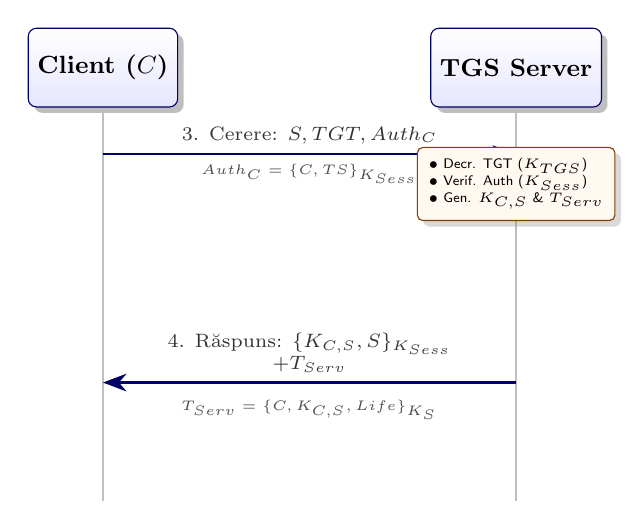
\begin{tikzpicture}[
        node distance=3.2cm, % Distanță compactă
        % --- DEFINIȚII DE STIL (Aici e magia design-ului) ---
        % 1. Actorii (Client/Server): Gradient Albastru + Umbră
        entity/.style={
                draw=blue!40!black,
                top color=white,
                bottom color=blue!10,
                rounded corners=3pt,
                align=center,
                minimum height=1cm,
                minimum width=1.8cm,
                drop shadow,
                font=\bfseries\small
            },
        % 2. Mesajele de pe săgeți
        msg/.style={
                midway,
                above,
                font=\scriptsize,
                color=black!80
            },
        % 3. Notele Interne (Chenarul cerut): Galben pal + Border Portocaliu
        process/.style={
                draw=orange!50!black,
                fill=orange!5,
                rounded corners=2pt,
                align=left,
                font=\tiny\sffamily, % Font sans-serif pentru cod/tehnic
                inner sep=4pt,
                drop shadow={opacity=0.3}
            },
        % 4. Formulele Matematice de sub săgeți
        mathnote/.style={
                below=0.1cm,
                font=\tiny,
                color=black!70
            }
    ]

    % 1. Actorii
    \node[entity] (client) {Client ($C$)};
    \node[entity, right=of client] (tgs) {TGS Server};

    % 2. Liniile vieții
    \draw[thick, gray!50] (client) -- ++(0,-5.5) coordinate (c_end);
    \draw[thick, gray!50] (tgs) -- ++(0,-5.5) coordinate (tgs_end);

    % 3. Mesajul 3 (Cerere)
    \draw[-{Stealth[length=3mm]}, thick, color=blue!40!black]
    ($(client)+(0,-1.1)$) --
    node[msg] {3. Cerere: $S, TGT, Auth_C$}
    ($(tgs)+(0,-1.1)$);

    % Formula Auth
    \node[mathnote] at ($(client)!0.5!(tgs) + (0,-1)$) {
    $Auth_C = \{C, TS\}_{K_{Sess}}$
    };

    % --- CHENARUL CERUT (Procesare Internă) ---
    % Folosim stilul 'process' definit mai sus
    \node[process, below=0.5cm of tgs, anchor=north] {
        $\bullet$ Decr. TGT ($K_{TGS}$)\\
        $\bullet$ Verif. Auth ($K_{Sess}$)\\
        $\bullet$ Gen. $K_{C,S}$ \& $T_{Serv}$
    };

    % 4. Mesajul 4 (Răspuns)
    \draw[-{Stealth[length=3mm]}, thick, color=blue!40!black]
    ($(tgs)+(0,-4)$) --
    node[msg, align=center] {4. Răspuns: $\{K_{C,S}, S\}_{K_{Sess}}$ \\ $+ T_{Serv}$}
    ($(client)+(0,-4)$);

    % Formula T_Serv
    \node[mathnote] at ($(client)!0.5!(tgs) + (0,-4)$) {
    $T_{Serv} = \{C, K_{C,S}, Life\}_{K_S}$
    };

\end{tikzpicture}

        }
        \caption{Fluxul TGS Exchange}
      \end{figure}
    \end{column}

  \end{columns}
  % --- SFÂRȘIT COLOANE ---

\end{frame}

\begin{frame}{Faza 3: Accesarea Serviciului (Client-Server)}

  \begin{columns}[c] % Aliniere verticală pe centru

    % --- COLOANA STÂNGA (Text) ---
    \begin{column}{0.5\textwidth}
      \begin{itemize}
        \item \textbf{Scop:} Accesul efectiv la resursa dorită.
        \item \textbf{Mecanism:} Clientul prezintă serverului:
              \begin{itemize}
                \item \textbf{Tichetul de Serviciu} ($T_{Serv}$).
                \item Un nou Authenticator pentru a dovedi identitatea.
              \end{itemize}
      \end{itemize}

      \vspace{0.3cm}

      % Blocul Stateless - Punct cheie
      \begin{block}{Rezultat: Sistem Stateless}
        Serverul acceptă cererea și validează tichetul local, \textbf{fără a comunica cu KDC-ul}.

        KDC-ul nu este interogat la fiecare accesare, asigurând scalabilitatea.
      \end{block}
    \end{column}

    % --- COLOANA DREAPTA (Diagrama) ---
    \begin{column}{0.5\textwidth}
      \begin{figure}
        \centering
        % Scalăm diagrama la lățimea coloanei
        \resizebox{\linewidth}{!}{%
          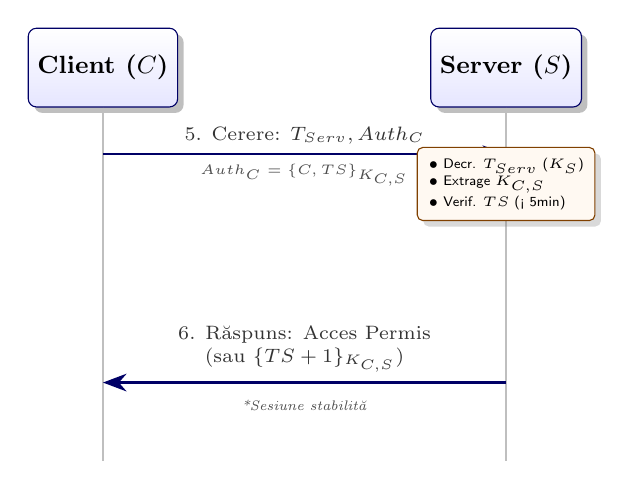
\begin{tikzpicture}[
        node distance=3.2cm, % Același spațiere compactă
        % --- STILURI (Identice cu celelalte figuri) ---
        entity/.style={
                draw=blue!40!black,
                top color=white,
                bottom color=blue!10,
                rounded corners=3pt,
                align=center,
                minimum height=1cm,
                minimum width=1.8cm,
                drop shadow,
                font=\bfseries\small
            },
        msg/.style={
                midway,
                above,
                font=\scriptsize,
                color=black!80
            },
        process/.style={
                draw=orange!50!black,
                fill=orange!5,
                rounded corners=2pt,
                align=left,
                font=\tiny\sffamily,
                inner sep=4pt,
                drop shadow={opacity=0.3}
            },
        mathnote/.style={
                below=0.1cm,
                font=\tiny,
                color=black!70
            }
    ]

    % 1. Actorii
    \node[entity] (client) {Client ($C$)};
    \node[entity, right=of client] (server) {Server ($S$)};

    % 2. Liniile vieții
    \draw[thick, gray!50] (client) -- ++(0,-5) coordinate (c_end);
    \draw[thick, gray!50] (server) -- ++(0,-5) coordinate (s_end);

    % 3. Mesajul 5 (Cerere Acces)
    \draw[-{Stealth[length=3mm]}, thick, color=blue!40!black]
    ($(client)+(0,-1.1)$) --
    node[msg] {5. Cerere: $T_{Serv}, Auth_C$}
    ($(server)+(0,-1.1)$);

    % Formula Auth
    \node[mathnote] at ($(client)!0.5!(server) + (0,-1)$) {
    $Auth_C = \{C, TS\}_{K_{C,S}}$
    };

    % --- CHENAR PROCESARE INTERNĂ SERVER ---
    % Am adăugat '\\' la final de rând pentru a forța verticalitatea
    \node[process, below=0.5cm of server, anchor=north] {
        $\bullet$ Decr. $T_{Serv}$ ($K_S$)\\
        $\bullet$ Extrage $K_{C,S}$\\
        $\bullet$ Verif. $TS$ (< 5min)
    };

    % 4. Mesajul 6 (Confirmare / Acces)
    \draw[-{Stealth[length=3mm]}, thick, color=blue!40!black]
    ($(server)+(0,-4)$) --
    node[msg, align=center] {6. Răspuns: Acces Permis \\ (sau $\{TS+1\}_{K_{C,S}}$)}
    ($(client)+(0,-4)$);

    % Notă finală
    \node[mathnote] at ($(client)!0.5!(server) + (0,-4)$) {
        \textit{*Sesiune stabilită}
    };

\end{tikzpicture}
        }
        \caption{Fluxul Client-Server}
      \end{figure}
    \end{column}

  \end{columns}

\end{frame}

\begin{frame}{Replicare și Disponibilitate}

  \begin{columns}[c]
    \begin{column}{0.5\textwidth}
      \begin{itemize}
        \item \textbf{Arhitectura:} Tip \textbf{Master-Slave}.
        \item \textbf{Master KDC:}
              \begin{itemize}
                \item Deține copia autoritativă (Read-Write).
                \item Singurul care acceptă scrieri (ex: schimbarea parolei).
              \end{itemize}
        \item \textbf{Slave KDCs:}
              \begin{itemize}
                \item Dețin copii Read-Only actualizate periodic.
                \item Asigură \textbf{disponibilitatea} în rețea.
              \end{itemize}
      \end{itemize}
    \end{column}

    \begin{column}{0.5\textwidth}
      \begin{figure}
        \centering
        \resizebox{\linewidth}{!}{%
          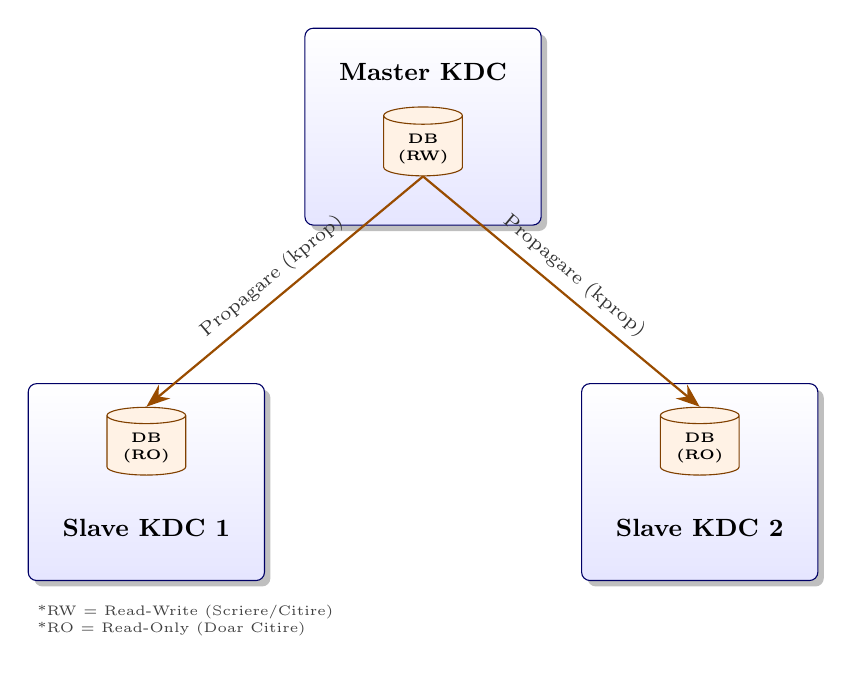
\begin{tikzpicture}[
    node distance=2cm,
    % --- STILURI (Păstrate din conversația anterioară) ---
    kdc/.style={
            draw=blue!40!black,
            top color=white,
            bottom color=blue!10,
            rounded corners=3pt,
            align=center,
            minimum height=2.5cm, % Dimensiunea mare
            minimum width=3cm,
            drop shadow,
            font=\bfseries\small
        },
    db/.style={
            cylinder,
            shape border rotate=90,
            draw=orange!50!black,
            fill=orange!10,
            aspect=0.25,
            minimum height=0.8cm,
            minimum width=1cm,
            font=\tiny\bfseries,
            align=center
        },
    propArrow/.style={
    -{Stealth[length=3mm]},
    thick,
    color=orange!60!black
    },
    msg/.style={
            midway,
            font=\scriptsize,
            color=black!80,
            sloped
        }
    ]

    % 1. Nodul MASTER - Textul urcat folosind spațiu gol dedesubt
    \node[kdc] (master) {Master KDC\\[1.0cm]};

    % Baza de date poziționată sub bordura de sus (north) a master-ului
    % Am ajustat la 1.1cm pentru a pica exact sub text
    \node[db, below=1.0cm of master.north] (masterDB) {DB\\(RW)};

    % 2. Nodurile SLAVE
    \node[kdc, below left=2cm and 0.5cm of master] (slave1) {\\[1.0cm]Slave KDC 1};
    \node[db, below=0.3cm of slave1.north] (slave1DB) {DB\\(RO)};

    \node[kdc, below right=2cm and 0.5cm of master] (slave2) {\\[1.0cm]Slave KDC 2};
    \node[db, below=0.3cm of slave2.north] (slave2DB) {DB\\(RO)};

    % 3. Conexiuni
    \draw[propArrow] (masterDB.south) -- node[msg, above] {Propagare (kprop)} (slave1DB.north);
    \draw[propArrow] (masterDB.south) -- node[msg, above] {Propagare (kprop)} (slave2DB.north);

    % Legendă
    \node[below=0.5cm of slave1.south west, anchor=west, font=\tiny, color=darkgray, align=left] {
        *RW = Read-Write (Scriere/Citire)\\
        *RO = Read-Only (Doar Citire)
    };

\end{tikzpicture}
        }
        \caption{Arhitectura de Replicare}
      \end{figure}
    \end{column}
  \end{columns}

\end{frame}

\begin{frame}{Analiză Teoretică: Corectitudine și Complexitate}
  \small % Micșorăm puțin fontul pentru a încăpea tot textul

  % Blocul 1: Analiza Corectitudinii
  \begin{block}{Corectitudine și Dependențe}
    \begin{itemize}
      \item \textbf{Sincronizarea Ceasurilor (Time Skew):}
            Deoarece protocolul se bazează pe \textit{Timestamp-uri} pentru a preveni atacurile, este critică sincronizarea prin NTP. O deviație $>5$ minute duce la respingerea tichetelor.
      \item \textbf{Integritatea KDC (TTP):}
            Securitatea este centralizată. Compromiterea cheii Master a KDC-ului permite crearea de \textit{"Golden Tickets"} (impersonare totală).
    \end{itemize}
  \end{block}

  \vspace{0.2cm} % Spațiu redus (era 0.5cm)

  % Blocul 2: Analiza Performanței
  \begin{block}{Performanță și Eficiență}
    \begin{itemize}
      \item \textbf{Complexitate de Rețea:} $\mathcal{O}(1)$.
            Protocolul necesită un număr constant de mesaje (\textbf{6 pachete}), indiferent de numărul de utilizatori.
      \item \textbf{Eficiență Computațională:}
            Utilizează exclusiv \textbf{criptare simetrică} (AES/DES), care este mult mai rapidă decât cea asimetrică (RSA), reducând încărcarea pe CPU.
    \end{itemize}
  \end{block}

\end{frame}

\begin{frame}{Topologii Avansate (1/2): Cross-Realm Authentication}
  \small % Revenim la \small, acum avem loc

  % 1. Blocul Problemă pe toată lățimea (sus)
  \begin{block}{Problemă: Limitarea KDC-ului Unic}
    Într-o companie globală, gestionarea tuturor utilizatorilor într-o singură bază de date este imposibilă (latenta rețelei, gât de sticlă).
  \end{block}

  \vspace{0.3cm}

  % 2. Coloane Inegale (Jos)
  \begin{columns}[c] % Aliniere verticală pe centru

    % --- COLOANA STÂNGA (40%) - Soluția și Pașii ---
    \begin{column}{0.4\textwidth}
      \textbf{Soluție:} Cross-Realm Authentication.

      \vspace{0.2cm}
      \textbf{Fluxul de operare:}
      \begin{enumerate}
        \item Client (Realm A) cere acces în Realm B.
        \item KDC A emite un \textbf{"Remote TGT"}.
        \item KDC B validează TGT-ul și emite tichetul.
      \end{enumerate}
    \end{column}

    % --- COLOANA DREAPTA (60%) - Diagrama ---
    \begin{column}{0.6\textwidth}
      \begin{figure}
        \centering
        % Diagrama se va scala la lățimea coloanei (60% din slide)
        % sau maxim 60% din înălțime, ca să nu iasă din pagină
        \resizebox{\linewidth}{!}{%
          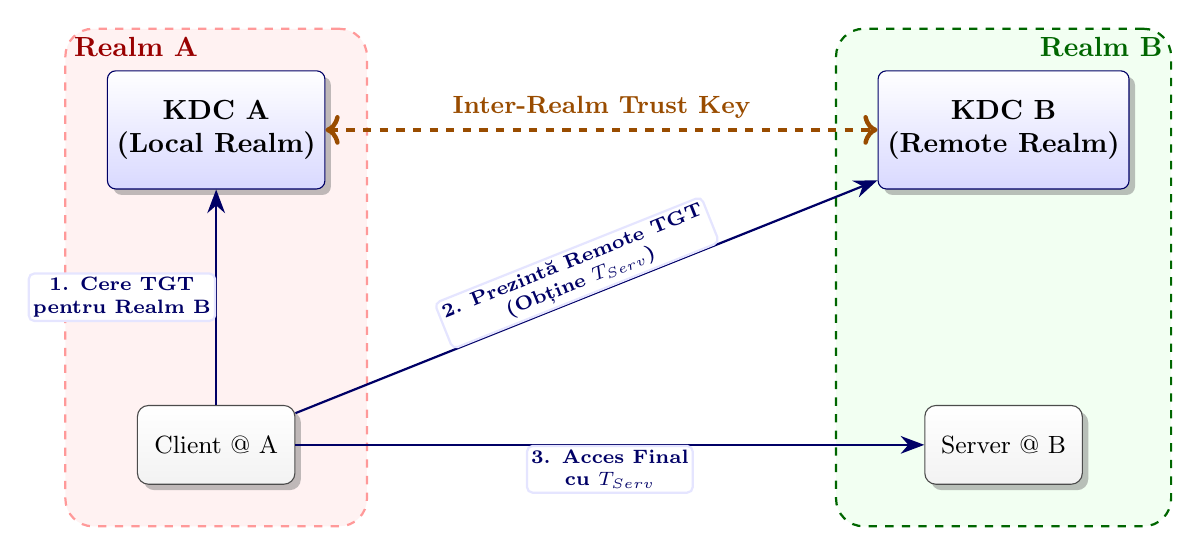
\begin{tikzpicture}[
    node distance=2.5cm,
    % --- STILURI VIZUALE ---
    kdc/.style={
            draw=blue!40!black,
            top color=white,
            bottom color=blue!15,
            rounded corners=3pt,
            align=center,
            minimum height=1.5cm,
            minimum width=2.5cm,
            drop shadow,
            font=\bfseries
        },
    entity/.style={
            draw=gray!60!black,
            top color=white,
            bottom color=gray!10,
            rectangle,
            rounded corners,
            minimum height=1cm,
            minimum width=2cm,
            align=center,
            drop shadow,
            font=\small
        },
    flow/.style={
    ->,
    >={Stealth[length=3mm]},
    thick,
    color=blue!40!black,
    rounded corners
    },
    lbl/.style={
            midway,
            fill=white,
            inner sep=1.5pt,
            font=\scriptsize\bfseries,
            text=blue!40!black,
            align=center,
            draw=blue!10,
            rounded corners=2pt
        },
    realm/.style={
            draw,
            dashed,
            rounded corners=10pt,
            inner sep=15pt,
            thick
        }
    ]

    % --- POZIȚIONARE NODURI ---
    % REALM A (Stânga)
    \node[kdc] (kdcA) at (0, 4) {KDC A\\(Local Realm)};
    \node[entity] (client) at (0, 0) {Client @ A};

    % REALM B (Dreapta)
    \node[kdc] (kdcB) at (10, 4) {KDC B\\(Remote Realm)};
    \node[entity] (server) at (10, 0) {Server @ B};

    % --- FUNDALURI REALMURI ---
    \begin{scope}[on background layer]
        \node[realm, draw=red!40, fill=red!5, fit=(kdcA) (client)] (boxA) {};
        \node[anchor=north west, color=red!60!black, font=\bfseries] at (boxA.north west) {Realm A};

        \node[realm, draw=green!40!black, fill=green!5, fit=(kdcB) (server)] (boxB) {};
        \node[anchor=north east, color=green!40!black, font=\bfseries] at (boxB.north east) {Realm B};
    \end{scope}

    % --- CONEXIUNI ȘI FLUX CORECTAT ---

    % 0. TRUST LINK
    \draw[<->, dashed, ultra thick, color=orange!60!black] (kdcA) --
    node[midway, above, font=\bfseries\small, color=orange!60!black] {Inter-Realm Trust Key}
    (kdcB);

    % 1. Cerere TGT pentru Remote
    \draw[flow] (client) --
    node[lbl, left] {1. Cere TGT\\pentru Realm B}
    (kdcA);

    % 2. Prezentare TGT la KDC B
    \draw[flow] (client) --
    node[lbl, sloped, above] {2. Prezintă Remote TGT\\(Obține $T_{Serv}$)}
    (kdcB);

    % 3. Acces Final (CORECTAT: Client -> Server, nu KDC -> Server)
    % Tichetul este prezentat de Client
    \draw[flow] (client) --
    node[lbl, below] {3. Acces Final\\cu $T_{Serv}$}
    (server);

\end{tikzpicture}

        }
        \caption{Flux Cross-Realm}
      \end{figure}
    \end{column}

  \end{columns}

\end{frame}

\begin{frame}{Topologii Avansate (2/2): Delegare (Proxy)}
  \small

  % Blocul Problemă (Sus, toată lățimea)
  \begin{block}{Problemă: Accesul Indirect}
    Un serviciu intermediar (ex: \textit{Print Server}) trebuie să acceseze o resursă protejată \textbf{în numele utilizatorului}, dar nu deține parola acestuia.
  \end{block}

  \vspace{0.2cm}

  \begin{columns}[c]

    % --- COLOANA STÂNGA (Mai lată pentru text - 65%) ---
    \begin{column}{0.65\textwidth}
      \textbf{Soluție:} Proxy Tickets.

      \vspace{0.2cm}
      \textbf{Mecanism:}
      \begin{itemize}
        \item Utilizatorul emite un tichet special care \textbf{deleagă} drepturile sale către Print Server.
        \item Tichetul conține restricții (adresă IP, timp de viață scurt).
        \item Serviciul intermediar îl prezintă mai departe ca dovadă.
      \end{itemize}
    \end{column}

    % --- COLOANA DREAPTA (Mai îngustă pentru diagrama înaltă - 35%) ---
    \begin{column}{0.35\textwidth}
      \begin{figure}
        \centering
        % CHEIA SUCCESULUI: Scalăm după ÎNĂLȚIME, nu lățime!
        % ! la lățime înseamnă "păstrează proporția".
        % 0.6\textheight înseamnă "maxim 60% din înălțimea slide-ului"
        \resizebox{!}{0.40\textheight}{%
          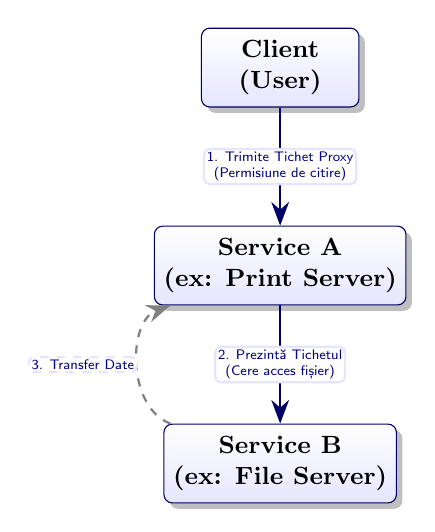
\begin{tikzpicture}[
    node distance=2.5cm,
    % --- STILURI (Compacte pentru o coloană) ---
    entity/.style={
            draw=blue!40!black,
            top color=white,
            bottom color=blue!10,
            rounded corners=3pt,
            align=center,
            minimum height=1cm,
            minimum width=2cm,
            drop shadow,
            font=\bfseries\small
        },
    flow/.style={
    ->,
    >={Stealth[length=3mm]},
    thick,
    color=blue!40!black
    },
    lbl/.style={
            midway,
            fill=white,
            inner sep=1pt,
            font=\tiny\sffamily,
            text=blue!50!black,
            align=center,
            draw=blue!10,
            rounded corners=2pt
        }
    ]

    % --- POZIȚIONARE PE VERTICALĂ (Flux Liniar) ---
    \node[entity] (client) {Client\\(User)};
    \node[entity, below=1.5cm of client] (print) {Service A\\(ex: Print Server)};
    \node[entity, below=1.5cm of print] (file) {Service B\\(ex: File Server)};

    % --- FLUX ---

    % 1. Client -> Print
    \draw[flow] (client) -- node[lbl] {1. Trimite Tichet Proxy\\(Permisiune de citire)} (print);

    % 2. Print -> File
    % Mică rafinare la text pentru precizie maximă
    \draw[flow] (print) -- node[lbl] {2. Prezintă Tichetul\\(Cere acces fișier)} (file);

    % 3. Confirmare
    \draw[flow, dashed, color=gray] (file) to[out=160, in=200] node[lbl, left] {3. Transfer Date} (print);

\end{tikzpicture}
        }
        \caption{Topologie Proxy}
      \end{figure}
    \end{column}

  \end{columns}

\end{frame}

\end{document}